\section{Експериментальні результати}\label{section2.1}

Для перевірки гіпотез на практиці було написано набір Python скриптів.
За основу взято відомий датасет текстур Бродатца \cite{brodatz} із фотографіями у відтінках сірого у однорідному освітленні.
Цей датасет використовується в тому числі для сумісності результатів із іншими науковими роботами.
Спочатку з оригінального датасету утворено тренувальні та тестові вибірки у потрібному форматі.
Далі проведено перевірку деяких сформульованих в роботі статистичних гіпотез для цієї вибірки.
Потім підготовлено статистичну модель для класифікації текстур декількома методами і оцінено їх ефективність.

\subsection{Підготовка даних}\label{section2.1a}

\begin{figure}[h]
    \centering
    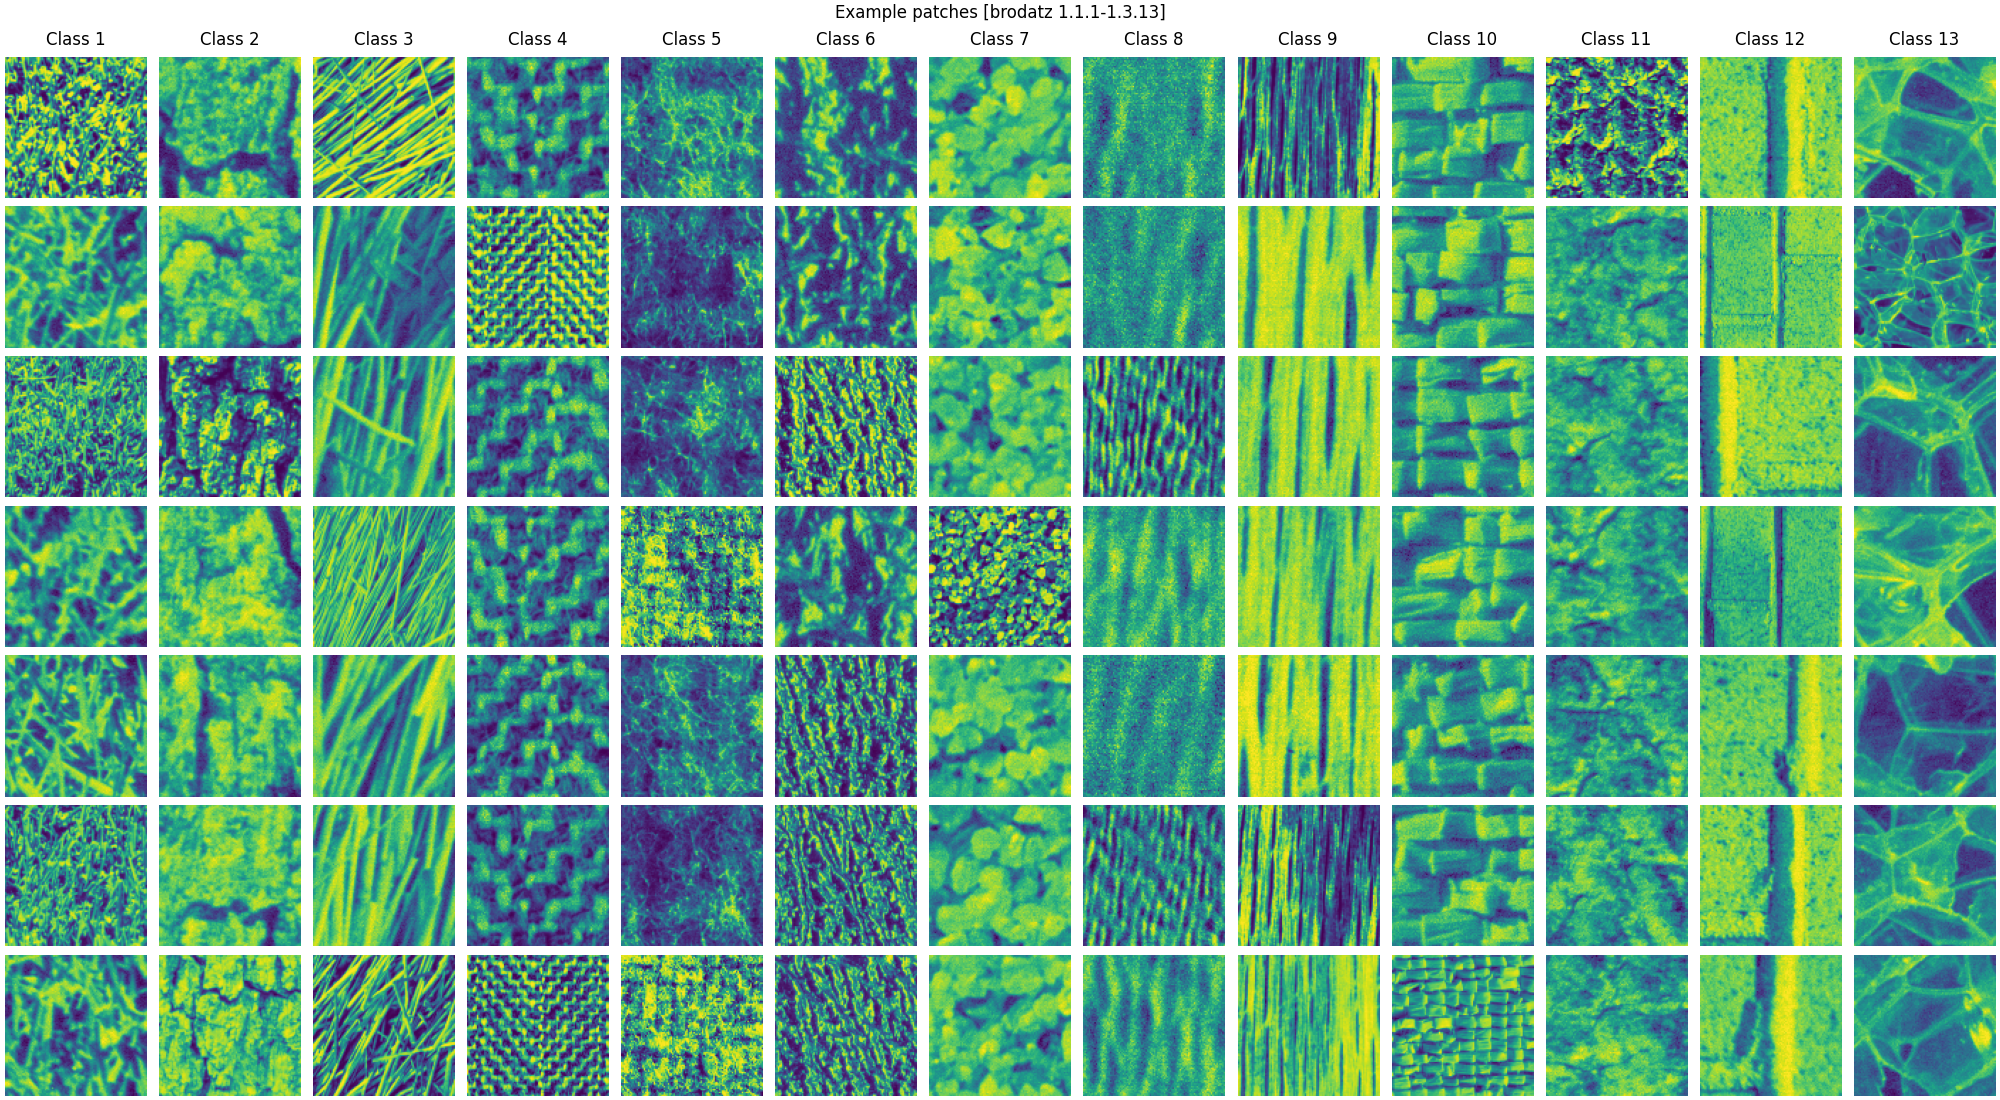
\includegraphics[width=0.99\textwidth]{img/example_classes.png}
    \caption{
        Приклад патчів $100\times 100$ у відтінках сірого, утворених з датасету текстур Бродатца; для кожного з типів текстур у наборі.
        Візуалізовано у псевдокольорах.
    }
    \label{fig:brodatz-showcase}
\end{figure}

У роботі використано перші три частини датасета Бродатца, які містять фотографії текстур у відтінках сірого у великому наближенні, всього 39 різних фотографій.
Датасет включає як однорідні та регулярні текстури (цегла, тканина), так і псевдорегулярні (дерево, кора, трава, сіно, шкіра). 
Кожна частина складається з 13-ти фотографій різних текстур (природних та штучних), при чому послідовність текстур повторюється між частинами. 
Зображення у перших двох частинах мають розміри 512 на 512 пікселів. 
Третя частина містить фотографії в іншому масштабі та у розмірі 1024 на 1024 пікселів.
Оригінальні фотографії розрізано на неперетинні квадратні частини (патчі) розміром 100 на 100 пікселів (ігноруючи залишкові пікселі).
Кожному патчу призначено дві мітки: номер текстури (1--13), та номер фотографії цієї текстури, з якого патч походить (1--3).

Таким чином, робоча вибірка містить по 350 патчів з першої та другої частин, і 1300 патчів з третьої частини; всього 1950 елементів вибірки.
Всі текстури представлені у вибірці збалансовано, кожна має по 150 представників.

\subsection{LBP дескриптори}\label{section2.1b}

У якості дескрипторів у роботі будуть дескриптори LBP із різними параметрами R та P, у стандартному та ``рівномірному'' варіантах.
Для сумісності результатів із попередніми дослідженнями \cite{ojala2002,fastlbp2024}, обрано наступні параметри:
(R=1,P=8), (R=2,P=12), (R=1,P=8, ``рівномірний''), (R=2,P=12, ``рівномірний''), (R=3,P=24, ``рівномірний''), (R=5,P=36, ``рівномірний'').
Кожному дескриптору відповідає вектор ознак, що обчислюється як гістограма значень дескриптора на зображенні (послідовність частот $\nu^{(T)}_d(I)$).
Для кожного патчу обчислено всі вектори ознак (наприклад, рис.~\ref{fig:example-features}).

\begin{figure}[h]
    \centering
    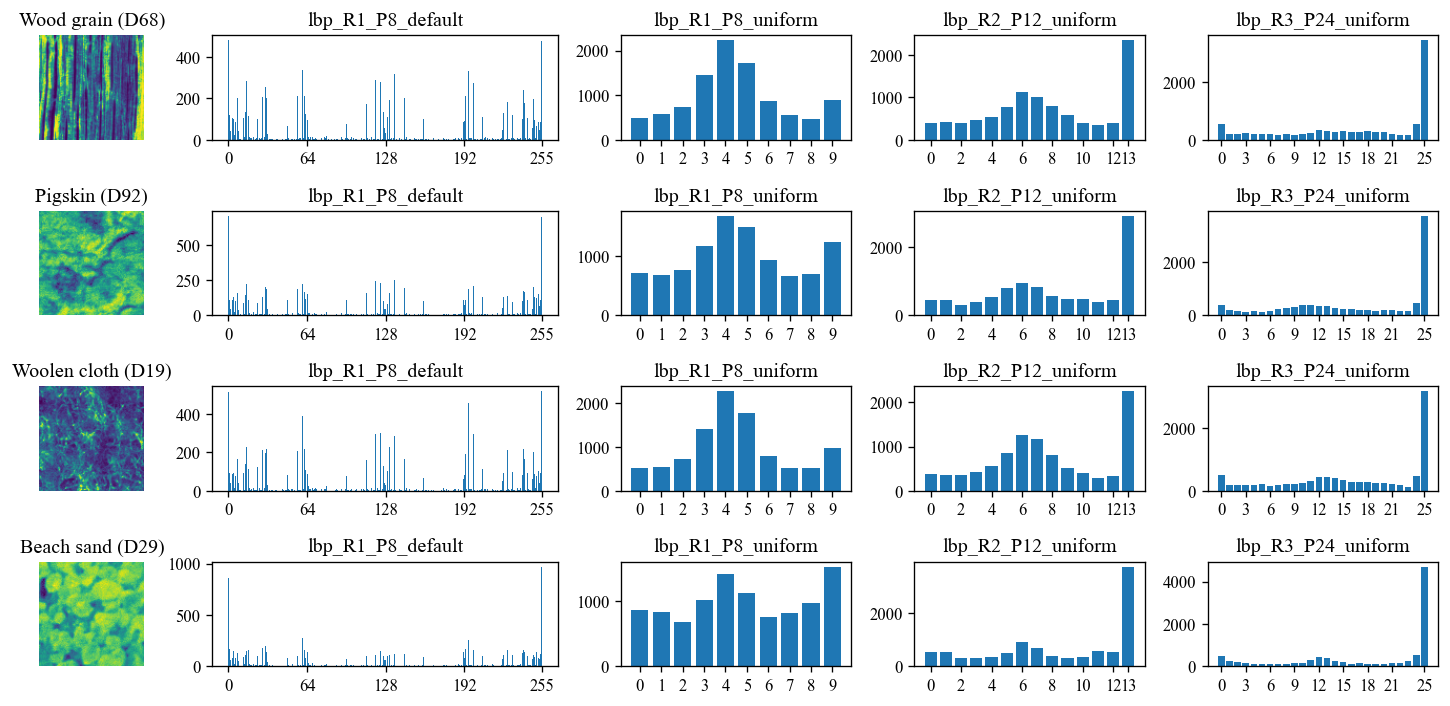
\includegraphics[width=0.99\textwidth]{img/example_features.png}
    \caption{
        Приклад деяких векторів ознак (гістограм) для деяких патчів
    }
    \label{fig:example-features}
\end{figure}

Для не-рівномірних дескрипторів стає суттєвою невелика кількість пікселів у патчі $100\times 100$.
Дескриптор R1P8 приймає 256 можливих значень і багато з них приймає рідко -- гістограма цього дескриптора містить медіанно 33\% частот менше 5, мінімально 15\% .
Дескриптор R2P12 приймає 4096 можливих значень і практично всі з них приймає рідко -- медіанно 92\% частот менше 5, мінімально 90\% .

Малі значення частот викривляють результати вищезгаданих статистичних тестів і збільшують залежність результату від точності обчислень.
Має сенс розділити множину значень дескриптора на $B$ рівних інтервалів, обираючи $B$ таким чином, щоб кількість малих частот була не більше, наприклад, 5\% \cite{ojala2002}.

Для мого датасету шляхом перебору виявилося, що 64 це гарна кількість інтервалів для R1P8. 
Це відповідає об'єднанню початкових 256 інтервалів по 4. 
За цих умов не більше 1,6\% нових інтервалів матимуть менш ніж 5 спостережень.
Для R2P12 гарною кількістю інтервалів виявилось 90. 
Це відповідає об'єднанню початкових 4096 інтервалів по 46. 
За цих умов не більше 5\% нових інтервалів матимуть менш ніж 5 спостережень.

Значення у гістограмах, що відповідають ``рівномірним'' дескрипторам LBP, не були об'єднані в інтервали, 
оскільки кількість різних значень на порядки менша за кількість спостережень і проблем із малими частотами не було.

\subsection{Статистична гіпотеза нормальності відхилень гістограми}\label{section2.1c1}

Для цього обчислено відхилення кожного вектору ознак від середнього значення серед інших векторів цього класу текстури.
Використано критерій нормальності Шапіро-Вілка (\verb|scipy.stats.shapiro|) окремо для кожної координати вектору ознак із значущостю 0,05.
Обчислено частку ймовірно не-нормально розподілених координат вектора у кожному класі текстур, а потім медіану по всім класам текстур.

Отримані результати зображено на рис.~\ref{fig:normaltest}. 
Бачимо, що в цілому не можемо припускати, що гістограми розподілено нормально навколо середньої у кожному класі.
Цікаво, що нормальність суттєво вища для ознак, утворених розбиттям гістограми на інтервали (reb\_hist\_R1\_P8\_d та reb\_hist\_R2\_P12\_d).

\begin{figure}[h]
    \centering
    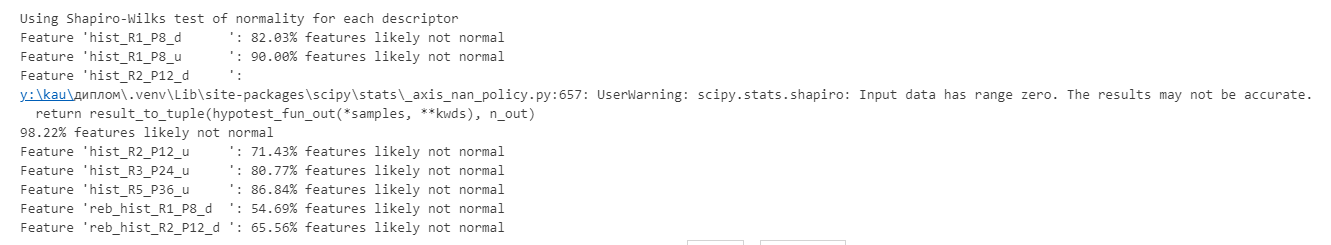
\includegraphics[width=0.99\textwidth]{img/normality-test.png}
    \caption{
        Результати застосування критерію нормальності 
    }
    \label{fig:normaltest}
\end{figure}

Також перевірено нормальність враховуючи те, що патчі були взяті з різних зображень із різними масштабами (рис.~\ref{fig:normaltest-subsets}).
Бачимо, що всередині підмножини вибірки нормальність значно вища.
Це може свідчити про те, що у загальній вибірці всередині класу маємо деяку суміш розподілів.
Таким чином, патчі з різних зображень одного типу текстури ймовірно мають суттєво різні розподіли, що необхідно враховувати при проєктуванні класифікаторів.
Ця гіпотеза буде перевірена глибше у наступних розділах.

\begin{figure}[h]
    \centering
    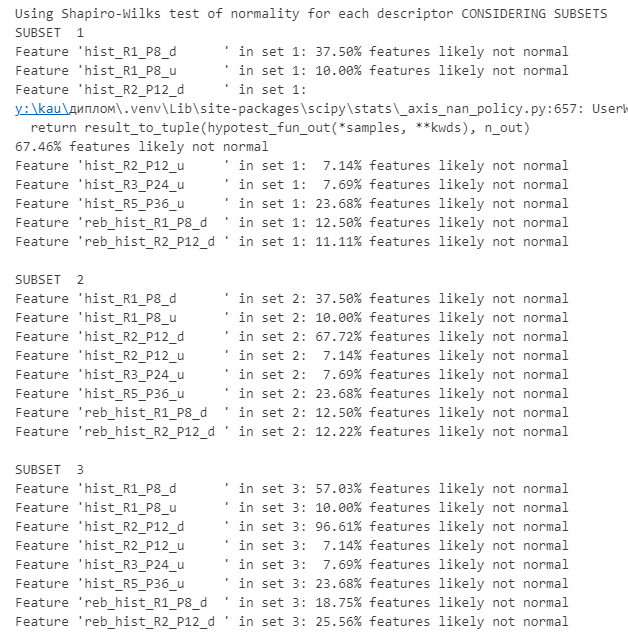
\includegraphics[width=0.5\textwidth]{img/normality-test-subsets.png}
    \caption{
        Результати застосування критерію нормальності із врахуванням підмножин вибірки
    }
    \label{fig:normaltest-subsets}
\end{figure}


\subsection{Статистична гіпотеза близькості середніх розподілів}\label{section2.1c2}

Якщо моделювати текстуру як деякий розподіл, то класифікація текстур може виконуватись за близькістю 
спостережуваної гістограми до інших, еталонних гістограм. 
Для використання статистичних критеріїв близькості розподілів ми припускаємо, 
що спостережувана гістограма сама є реалізацією деякого розподілу, 
наприклад нормального розподілу із центром у середній гістограмі певного класа текстури.
У попередньому пункті перевірено, наскільки доцільно вважати цей розподіл нормальним.
У цьому пункті перевіримо, чи достатньо суттєво відрізняються середні гістограми класів текстур, щоб вважати, 
що відповідні текстури моделюються різними розподілами.

Для середніх гістограм кожної пари класів текстур було обчислено критерій близькості розподілів відношення log-правдоподібності (\verb|scipy.stats.power_divergence| із \verb|lambda_='log-likelihood'|). 
Спершу разом для всіх патчів датасету (рис.~\ref{subfig:distr-sim-all}), а потім враховуючи зображення, з якого походить патч (рис.~\ref{subfig:distr-sim-subsets}). 
В обох випадках прийнято рівень значущості 0,05. 

\begin{figure}[h]
    \begin{subfigure}{0.48\textwidth}
    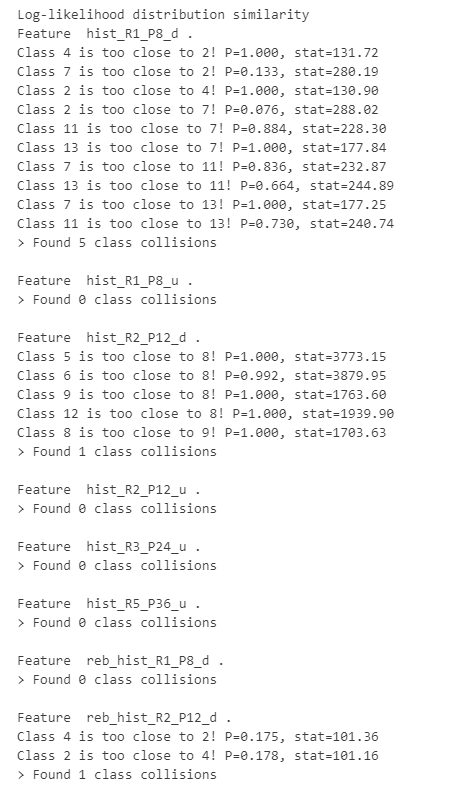
\includegraphics[width=0.9\linewidth]{img/distr-sim.png} 
    \caption{
        Результати критерію близькості розподілів для загальної вибірки.
    }
    \label{subfig:distr-sim-all}
    \end{subfigure}%
    \hfill
    \begin{subfigure}{0.48\textwidth}
    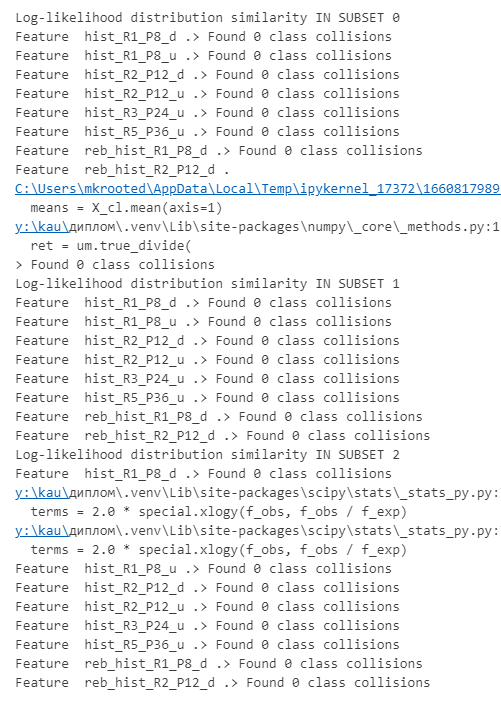
\includegraphics[width=0.9\linewidth]{img/distr-sim-subsets.png}
    \caption{
        Результати критерію близькості розподілів враховуючи зображення, з якого походять патчі. 
    }
    \label{subfig:distr-sim-subsets}
    \end{subfigure}
    
    \caption{}
    \label{fig:distr-sim}
\end{figure}

Бачимо, що у загальній вибірці лише стандартні дескриптори R1P8 та R2P12 ``плутають'' деякі класи; 
проте, це не спостерігається у вибірці, що враховує зображення, з яких походять патчі.
В обох випадках спостерігалися проблеми із нульовими частотами стандартного дескриптора R2P12 через його велику множину значень.
Таким чином, дійсно маємо підстави моделювати текстуру через розподіл значень дескриптора і можемо переходити до класифікації.

\subsection{Класифікація частково відомих текстур}\label{section2.1d}

Побудовано два класифікатора: примітивний класифікатор на основі близькості до середньої гістограми, 
та класифікатор за 3-ма найближчими сусідами із евклідовою метрикою (що грубо еквівалентно статистиці $\chi^2$ близкості розподілів).
Точність класифікації оцінюватимемо як середнє значення точності класифікації кожного класу текстури --
\begin{equation*}
    \text{precision} = \frac{1}{\# S} \sum_{s \in S} \sum_{I : \kappa(I) = s} \frac{\1(g(I) = s)}{\# \{I : \kappa(I) = s\}},
\end{equation*}
де $S$ -- множина класів текстури, $g(I)$ -- передбачений класифікатором клас, $\kappa(I)$ -- дійсний клас. 
Тобто точність обчислюється як частка правильно класифікованих патчів серед усіх патчів.
Для коректних результатів, точність класифікатора перевіряється лише на патчах, яких не було у тренувальній вибірці.
Тренувальна вибірка складається із випадково обраних 60\% патчів із загальної вибірки, не зважаючи на зображення, з якого утворені патчі.
Таким чином класифікатор вчиться і перевіряється на тих самих зображеннях, але різних їх частинах.
Класифікація виконується за кожним дескриптором окремо від інших.

Перший класифікатор побудовано за принципом, описаним у рівнянні~\eqref{e:gtest-classifier-1}, 
що відповідає пошуку найближчого середнього вектора згідно відстані Кульбака-Ляйблера.
Результати зображені на рис.~\ref{fig:precision-1}.
Найкраще показують себе стандартний LBP R1P8 дескриптор та дескриптори R1P8 й R2P12 із розбитими на інтервали гістограмами, проте не стандартний R2P12.
Об'єднання значень у інтервали підивщило точність класифікації для дескриптора із великою областю значень.
Рівномірні дескриптори в цілому показали гіршу точність класифікації.
Матриці невідповідностей на рис.~\ref{fig:precision-1} показують кількість патчів із класом рядка, які класифіковані класом стовпця. 

\begin{figure}[h]
    \begin{subfigure}{0.5\textwidth}
    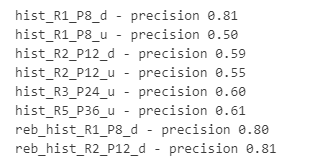
\includegraphics[width=0.95\linewidth]{img/precision-1.png} 
    \caption{
        Точність класифікації за~\eqref{e:gtest-classifier-1} для різних векторів ознак.
    }
    \end{subfigure}%
    \begin{subfigure}{0.5\textwidth}
    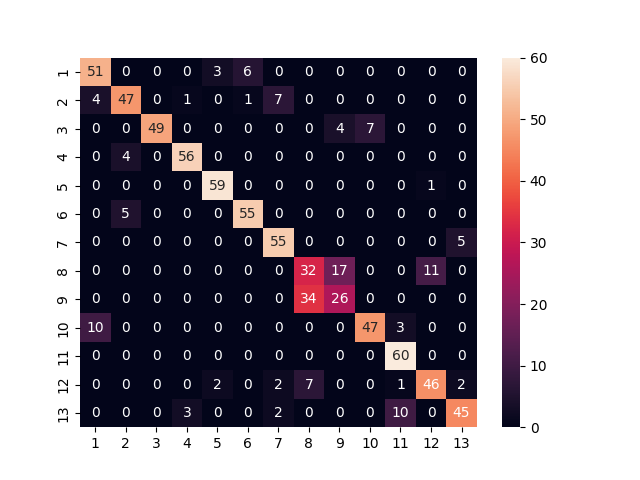
\includegraphics[width=0.95\linewidth]{img/confusion/hist_R1_P8_d.png}
    \caption{
        Матриця невідповідностей стандартного R1P8 (точність 0,81)
    }
    \end{subfigure}

    \begin{subfigure}{0.5\textwidth}
    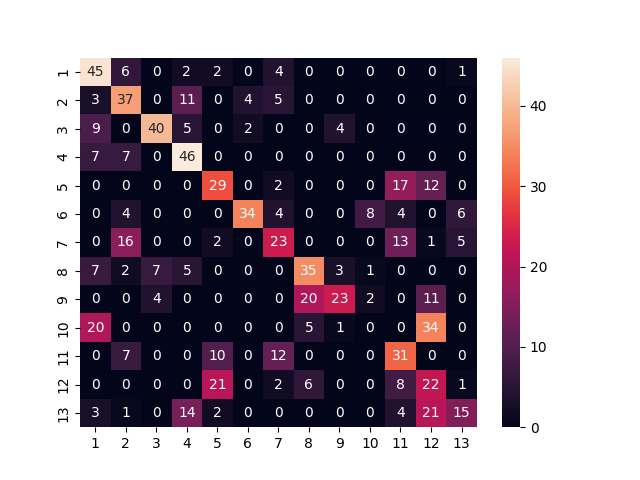
\includegraphics[width=0.95\linewidth]{img/confusion/hist_R1_P8_u.png}
    \caption{
        Матриця невідповідностей рівномірного R1P8 (точність 0,5)
    }
    \end{subfigure}%
    \begin{subfigure}{0.5\textwidth}
    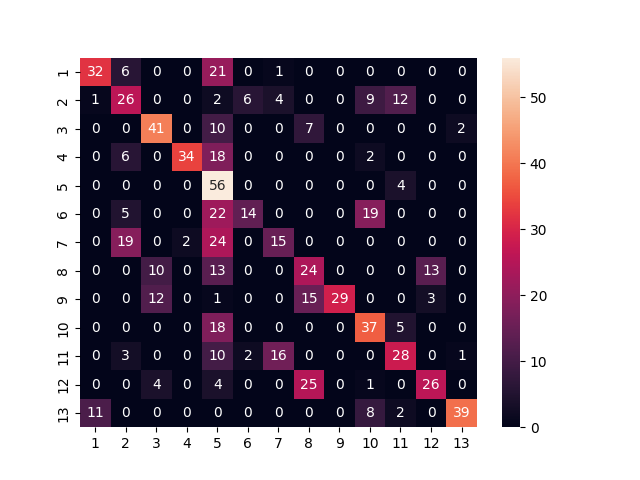
\includegraphics[width=0.95\linewidth]{img/confusion/hist_R5_P36_u.png}
    \caption{
        Матриця невідповідностей рівномірного R5P36 (точність 0,61) 
    }
    \end{subfigure}%
    
    \caption{Класифікатор за близкістю до середнього розподілу}
    \label{fig:precision-1}
\end{figure}

У всіх варіантах спостерігається близькість класів 8 та 9, що відповідають відповідно фотографіям поверхні води та дерев'яного зрізу,
які на око дійсно виглядають дещо схожими. 

Другий класифікатор побудовано на основі \verb|KNeighborsClassifier| з пакету SciPy із стандартною Евклідовою метрикою та трьома сусідами.
Результати зображено на рис.~\ref{fig:precision-2}. 
Точність класифікації з допомогою всіх дескрипторів вийшла досить висока.
Найкраща точність у стандартних дескрипторів R1P8 та R2P12, а
найгірше себе показав рівномірний дескриптор радіуса 5, при цьому будучи точнішим, за всі класифікатори першого типу.
Інші дескриптори призводять до приблизко однаково точної класифікації.

Важливим спостереженням є те, що рівномірні дескриптори використовують суттєво менші вектори ознак 
(не більше 40 координат, порівняно із 256 та 4096 координат для R1P8 та R2P12), 
але породжують всього незначно менш точні класифікатори.
Також цікаво, що KNN класифікатори набагато краще відрізняють навіть візуально схожі класи, які попередній класифікатор розрізняв погано.

\begin{figure}[h]
    \begin{subfigure}{0.5\textwidth}
    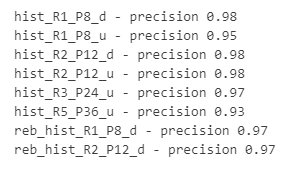
\includegraphics[width=0.95\linewidth]{img/precision-2.png} 
    \caption{
        Точність класифікації за KNN для різних векторів ознак.
    }
    \end{subfigure}%
    \begin{subfigure}{0.5\textwidth}
    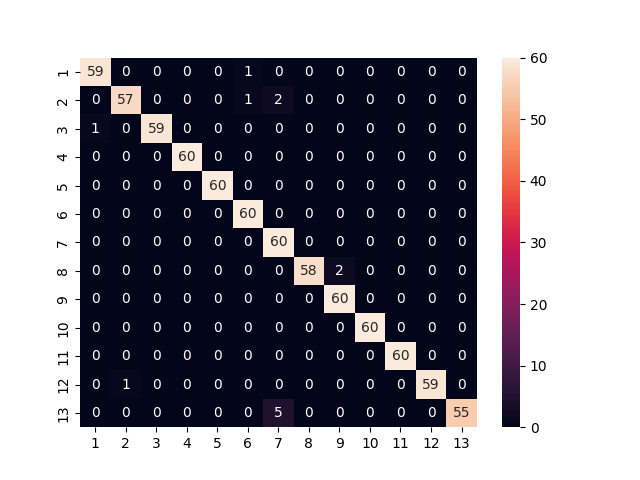
\includegraphics[width=0.95\linewidth]{img/confusion/knn-hist_R1_P8_d.png}
    \caption{
        Матриця невідповідностей стандартного R1P8 (точність 0,98)
    }
    \end{subfigure}

    \begin{subfigure}{0.5\textwidth}
    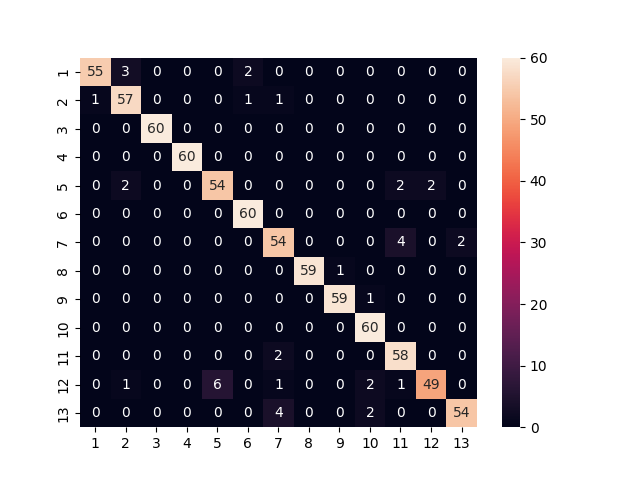
\includegraphics[width=0.95\linewidth]{img/confusion/knn-hist_R1_P8_u.png}
    \caption{
        Матриця невідповідностей рівномірного R1P8 (точність 0,95)
    }
    \end{subfigure}%
    \begin{subfigure}{0.5\textwidth}
    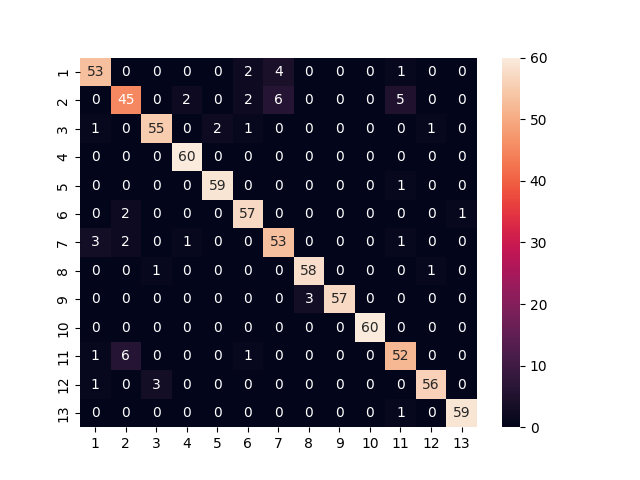
\includegraphics[width=0.95\linewidth]{img/confusion/knn-hist_R5_P36_u.png}
    \caption{
        Матриця невідповідностей рівномірного R5P36 (точність 0,93) 
    }
    \end{subfigure}%
    
    \caption{Класифікатор KNN}
    \label{fig:precision-2}
\end{figure}

\subsection{Класифікація невідомих текстур}\label{section2.1e}
Розділимо патчі за зображеннями, з яких вони походять.
Тренуватимемо класифікатори лише на частині патчів з одного зображення, оцінюватимемо на патчах з іншого.
Таким чином можемо перевірити, наскільки модель з одного представника текстури узагальнюється на інші представники.  
Важливо, що перша та друга фотографії мають однаковий масштаб, проте третя відрізняється масштабом приблизно у 2 рази.
У всіх випадках класифікатор навчається на випадкових 60\% патчах першого зображення, і оцінюється на всіх патчах другого та третього зображень.
Результати зібрано на рис.~\ref{fig:precision-3}.

Бачимо, що для зображень одного масштабу модель досить гарно узагальнюється для обох типів класифікаторів; 
і навіть показує кращий результат, ніж при тренуванні на всіх зображеннях.
З іншого боку, точність на зображенні більшого масштабу зрівнянна із вибором класу випадковим чином ($\frac{1}{13} \approx 0,08$), 
що свідчить про очікувану несумісність навчальних і тестових даних, тобто значну різницю у розподілах дескрипторів.
Цікаво, що найкраще узагальнюються моделі, побудовані на дескрипторах із розбиттям множини значень на інтервали.
Найгірше узагальнювалась модель на основі гістограм дескриптора із найбільшою множиною значень, R2P12.

\begin{figure}[h]
    \begin{subfigure}{0.5\textwidth}
    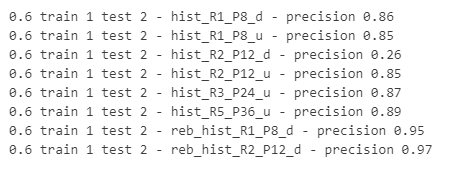
\includegraphics[width=0.95\linewidth]{img/precision-3.png} 
    \caption{
        Класифікатор на середніх гістограмах. Навчено на зображенні 1, перевірено на зображенні 2 того ж масштабу.
    }
    \end{subfigure}%
    \begin{subfigure}{0.5\textwidth}
    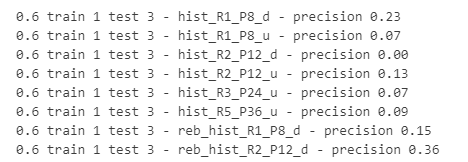
\includegraphics[width=0.95\linewidth]{img/precision-4.png}
    \caption{
        Класифікатор на середніх гістограмах. Навчено на зображенні 1, перевірено на зображенні 3 іншого масштабу.
    }
    \end{subfigure}

    \begin{subfigure}{0.5\textwidth}
    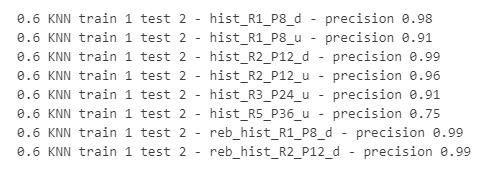
\includegraphics[width=0.95\linewidth]{img/precision-3-knn.png} 
    \caption{
        KNN класифікатор. Навчено на зображенні 1, перевірено на зображенні 2.
    }
    \end{subfigure}%
    \begin{subfigure}{0.5\textwidth}
    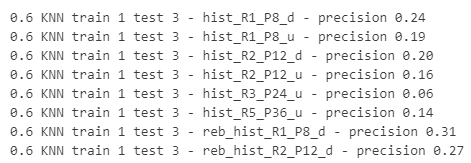
\includegraphics[width=0.95\linewidth]{img/precision-4-knn.png}
    \caption{
        KNN класифікатор. Навчено на зображенні 1, перевірено на зображенні 3.
    }
    \end{subfigure}
    
    \caption{}
    \label{fig:precision-3}
\end{figure}


\subsection{Висновки}\label{section2.1f}

Текстуру дійсно має сенс моделювати як розподіл значень деяких текстурних дескрипторів.
Утворена модель достатньо загальна, щоб описувати і інші реалізації текстури, проте лише схожих масштабів; 
моделі однієї текстури різних масштабів відрізняються.
Рівномірні LBP дескриптори дійсно описують текстуру достатньо повно: за умови правильно підібраного класифікатора, короткі вектори ознак від рівномірних дескрипторів можуть давати точність класифікації 
співставну із значно довшими ознаками від стандартних дескрипторів. 
Гістограми із великою кількістю комірок та великою кількістю малих частот є сенс згруповувати за інтервалами, що також призводить до кращої придатності моделі до узагальнення.
Класифікація за K найближчими сусідами призводила до точнішої класифікації у практично всіх випадках, а особливо у випадку якісно різних представників одного класу текстури.
